\documentclass[14pt]{extarticle}
\input{external/preamble-latex-cools.tex}
\begin{document}
\begin{project}{Actividad de cierre}{Regalitos para invitados.}{cool-regalitosInvitados}%
Clare tiene 48 marcadores. Ella pone 8 marcadores en cada bolsa de regalitos para su fiesta de cumpleaños. ¿Cuántas bolsas usará?%
\par
¿Cuál dibujo corresponde a la situación? Explica tu razonamiento.%
\begin{sidebyside}{2}{0}{0}{0}%
\begin{sbspanel}{0.5}%
A.%
\par
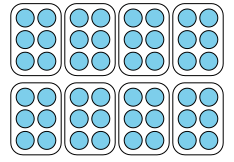
\includegraphics[max width=\linewidth, center]{external/svg-source/tikz-file-246306.pdf}
\end{sbspanel}%
\begin{sbspanel}{0.5}%
B.%
\par
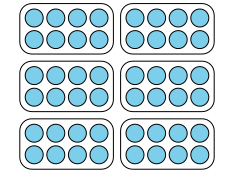
\includegraphics[max width=\linewidth, center]{external/svg-source/tikz-file-246307.pdf}
\end{sbspanel}%
\end{sidebyside}%
\begin{image}{0}{1}{0}{}%

\includegraphics[max width=\linewidth, center]{external/whitespace-tikz/2cm.pdf}
\end{image}%
\end{project}
\end{document}